\label{sectionVLC}
\begin{figure}[hbt]
	\centering
  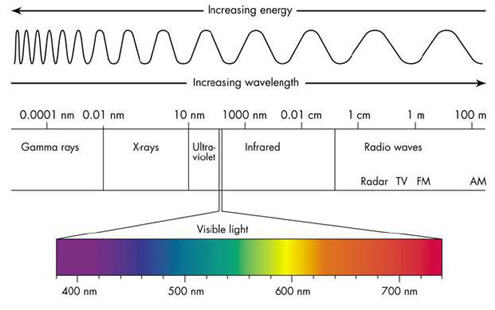
\includegraphics[height=200px]{img/wavelengths}
  \caption{Wavelengths, highlighted visible light band}
  \label{fig:wavelength}
\end{figure}

%intro
Visible Light Communication is a form of optical communication that uses signals in the visible light band to transmit information.
Contrary to the more common fiber-optic communication, VLC is wireless, and transmitted over free space.
In this context, for free space it is meant air, vacuum, or something similar, in contrast to other forms of optical communication that channel transmission into cables or others, like it is for fiber-optic.
Typically, normal fluorescent lamps or LEDs, rather than complex communication devices,  are used to transmit in VLC.
In general, receivers are electronic devices that include one or more photoresistors, in order to measure light signals from a source.
In some cases, digital cameras can also be used to as receivers, but it is a more challenging approach since the frame rate of modern video cameras is generally slow for communication, at around 30 - 60 Hz.
By modulating the light source through a controller it is possible to encode messages from digital form into light signals.
The simplest example of this encoding is a binary representation of data through light, where the presence of light represents a binary 1 and its absence a 0.
This form of communication is a simplified variation of the technology known as Li-Fi, a term that stands for Light-Fidelity.
LiFi and VLC in general can be used in pervasive computing applications, seeing the pervasiveness of light emitting devices everywhere.
Example of devices that could be enhanced with a communication feature are common lamps, both indoor and outdoors, car and traffic lights, commercial signs, even smartphones.
Visible light has been proven by research to achieve good transmission speeds and distances, is user friendly, safe, and easily restrained. 
\newline 
In general, \textbf{LED}s are the preferred light emitters in VLC systems.
The reasons can be several: LEDs can be pulsed at very high speeds without noticeable effect on the lighting and with no damage to the bulb, they last much longer than their competitors and require much less voltage and current.
Compared to halogen, incandescent or fluorescent light bulbs, LEDs do not use tungsten filaments that can get damaged.
Instead, they use a PN junction between two semiconductor materials that, when activated with a suitable voltage, realises energy in form of photons.
Since there is no filament to damage, LEDs can last much longer than other bulbs, and can undergo fast switching without danger.
\todo{maybe have some references here?}
 
 %optical
\subsection{Optical Communication}
Optical communication is allegedly one of the oldest types of communication from a distance in the history of human kind.
Examples of early communication techniques that use light to carry signals can be traced back millennia, with the first lighthouses, navigation lights, beacon fires that would assist in navigation or communicate danger.
It is only with the spread of electricity though, that optical communication technologies could really develop.
Many trace the start of Visible Light Technology back to 1880, when Alexander Graham Bell and Charles Sumner Tainter invented the photophone, a device able to transmit wireless voice messages over several hundred meters modulating sunlight. \todo{reference to photophone}
Since then, optical communication has been developed to include many different variants, the most common of which is \textbf{fiber optic communication}. 
This form of communication sends signals as light pulses through optical fiber.
Optical fiber is a hair-thin, transparent, extremely pure glass or plastic fiber that allows optical signals to travel from one end to the other with very high reliability\cite{opticalfiber}.
The light signal is constantly kept at the centre of the fiber, in its core.
Around the core, there is a layer called cladding, in a material of lower refractive index than the core.
This is to ensure that the light is trapped in the core, exploiting an optical property called total internal reflection.
All around the fiber there is a buffer layer, that protects the fiber itself.
Transmitters are usually LEDs or laser diodes, that can transmit in the visible light spectrum, infrared, or ultra violet.
Infrared light is more common however, because transmission is achieved with less attenuation and dispersion compared to visible light.
Fiber optic communication achieves high bandwidth, long distances, and is not subject to electromagnetic interference, contrary to electrical cabling.
Like fiber optics, also other common optical communication technologies include \textbf{infrared} light (IR) and \textbf{ultraviolet} (UV).
Infrared communication is used over free space to achieve short and long range communication.
As an example, most remote controllers use infrared signals, often modulated to to prevent interference form other light sources.
 
%indoor
\subsection{Indoor positioning}
In 2015, Philips released their LED based indoor positioning system as part of a collaboration with the supermarket chain Carrefour\cite{philps}.
The first installation has been delivered in one of their supermarkets in Lille, France.
Similar installations have been done for other retailers in D\"usselforf (Germany), Dubai (Emirates), and Eindhoven (Netherlands).
LED fixtures inside the shop transmit unique VLC signals that are received by smartphones through their front camera.
Paired with a cloud based database, the light signals are translated into a specific indoor position inside the shop, to help the user determine his/hers location.
To every product and offer in the shop is also associated a specific position inside the shop, conveniently displayed on a map for helping navigation and path finding. 
The system achieves illumination of the shop, energy saving for the lightning, and an indoor positioning system.
The system is intended for large retailers to assist shoppers find products and promotions faster, and navigate through the aisles, but can potentially be used in a wider range of applications.
For example it could be used in hospitals and elderly care facilities to track resources and people \cite{arduinobasedindoors}, or to assist/control indoor robotic vehicles in large warehouses.

%ronja
\subsection{RONJA}
RONJA (Reasonable Optical Near Joint Access) is a visible light communication system that operates wirelessly in free space using light beams that can achieve 10 Mbit/s full duplex Ethernet point-to-point link at 1.4 km of distance \cite{ronja}.
The entire system is labeled as User Controlled Technology: blueprints, schematic, building instructions and software components are all open source and freely available, the design is published under the GNU Free Documentation License.
It is a project originated in the Czech Republic and released in 2001 by Twibright Labs.
The group provides the instructions and the design of the system, leaving the purchase of the components and the assembly of the system to the end user.
In 2010 it has been estimated that up to 2000 links have been built worldwide \cite{ronjaestimation}.
Of the three official model designs, only two use visible light (red), while the third uses infrared.

%lifi
\subsection{Li-Fi}
The term Li-Fi was first introduced by a german physicist, Harald Haas, co-founder of PureLiFi, in occasion of a TED Global talk on Visible Light Communication in 2011 \cite{tedtalk}.
Since then, the term has been reported in many articles and has gained popularity as a common synonymous for Visible Light Communication.
After the name was adopted by the Optical Wireless Communication (OWC) community with the launch of the LiFi Consortium in 2011, an industry group that promotes OWC technologies, it can be sometimes extended to describe general wireless data access points that use light, visible or otherwise.
This includes also the infra-red and ultraviolet band.\\
The main reason why this technology is quickly gaining popularity in the research is because it potentially allows to unlock a vast amount of electromagnetic spectrum in the visible light region, unused for transmission.\cite{haas1}
This has been seen as a promising reaction to the saturation of the Radio Frequency (RF) spectrum, a very likely outcome of the huge success of wireless technology, also predicted by the US Federal Communication Commission\cite{crisis}. 
A second reason is that transmission through light can achieve surprising high speeds.
Starting from 2010, research had been able to improve the transmission rate further and further.
In his TED talk in 2011 Haas demonstrated real time video streaming from a white LED at data rates up to 130 Mbps\cite{tedtalk}, while another group achieved over 513 Mbps\cite{500Mbps}.
In the following years, there have been continuous reports of improved data rates in transmission.
A single white LED has been proven to transmit from about 1 Gbps\cite{1Gbps}, up to 3.5 Gbps\cite{3.5Gbps}, while 3.4 Gbps have been demonstrated with a single RGB LED\cite{3.4Gbps}.\\
This rates can be further improved by the use of arrays of light sources and more complex systems.
The Mexican software company Sisoft together with scientists from the Autonomous Technological
Institute of Mexico in 2014 reached the surprising data rate of 10 Gbps, setting the record.\\
Other appealing aspects to this technology are the low cost of implementation for the use of off-the-shelf LED bulbs and its security, for the reason that communication can be eavesdropped only in direct line of sight within short distance.\\
There are a few groups that are leading the research in the field of Visible Light Communication.
One of these is the Li-Fi R\&D Centre at the University of Edinburgh, of which prof. Harald Haas is the director.
Another very important research group operating in the same area is Disney Research, often in collaboration with ETH Zurich.
Another group worth mentioning is the Li-Fi Consortium, an international organisation formed by companies in optical wireless communication technology and research institutes.
A good part of the research is also carried out by multiple other research groups worldwide, especially in Asia and India in particular.

%standards
\subsection{Standard and specifications}
\label{modulschemes}
Visible light communication is regulated by a standard similar to the one of wireless networks, in the same IEEE 802 family.\cite{IEEE}
The IEEE 802.15.7 standard defines a draft of the physical layer (PHY) and the media access control (MAC) layer for VLC. 
According to Gordon Povey, former CEO at PureLiFi\cite{poveyspec}, the MAC layer as of April 2011 supports three multiple access topologies: peer-to-peer, star configuration and broadcast mode.\\
The Physical layer is divided into three types, that use different modulation schemes.
The three modulation schemes are: 
\begin{itemize}
\item On-Off Keying
\item Variable pulse position modulation (VPPM)
\item Colour shift keying (CSK)
\end{itemize}
\textbf{On-Off Keying}\newline
On-Off Keying is the simplest modulation scheme. 
In this scheme, a digital 1 is represented by the light state being on, and 0 otherwise.
In the 802.15.7 standard, Manchester coding is used to ensure the period of each pulse is the same.
This type of encoding, instead of having a digital 0 represented by a low signal and a digital 1 by a high signal, encodes each data bit as either low then high (1), or high then low (0), in equal time.\\
\newline
\begin{figure}[H]
\centering
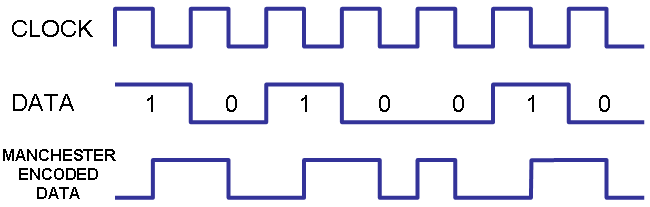
\includegraphics[scale=0.3]{img/ookmodulation}
\caption{OOK modulation using Manchester coding.}
\label{fig:ookmod}
\end{figure}
\textbf{Variable pulse position modulation (VPPM)}\newline
VPPM is similar to pulse position modulation (PPM), in which the data is encoded using the position of the pulse within a set time period.
In this modulation scheme, light dimming is allowed as long as the period containing the pulse is long enough to allow different positions to be identified. 
As in the Manchester coding a positive pulse at the beginning of the period followed by a negative pulse at the end can represent a digital 0, and a 1 is represented by a negative pulse at the beginning followed by a positive one at the end.\\
\newline
\begin{figure}[H]
\centering
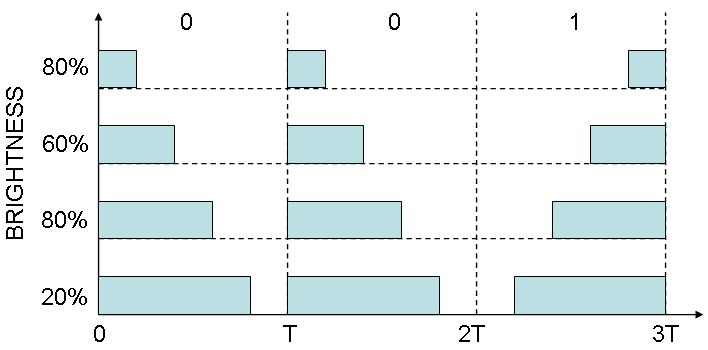
\includegraphics[scale=0.3]{img/VPPM}
\caption{Variable pulse position modulation to support light dimming.}
\label{fig:ookmod}
\end{figure}
\textbf{Colour shift keying (CSK)}\newline
This scheme allows the light intensity to be constant by encoding the information in the colour of the light.
For implementing this kind of transmission the system must use RGB type LEDs.

%other technologies
\subsection{Comparison with other technologies}
In this section, a comparison between common wireless technologies in relation to VLC is presented.
The data is partially based on the article "Comparative Performance Analysis of Wireless
Communication Protocols for Intelligent Sensors
and Their Applications" (2014) \cite{comparison}.\\
\newline
  \begin{tabular}{l| c c c c}
    Technology & frequency band & range & max. data rate & source localisation\\
    \hline
   WiFi & 2.4 GHz / 5 GHz & 10-100 m &  54 Mbps & no\\
   Bluetooth & 2.4 GHz & 10-100 m & 1-3 Mbps & no \\
   UWB & 3.1 - 10.6 GHz & 10-100 m & 110 Mbps & no\\
   ZigBee & 0.8 - 2.4 GHz & 10-1000 m &  250 Kbps & no\\
   Mobile broadband 3G & 0.85/ 0.9/ 2.1 GHz & 2-35 km &  2-21.6 Mbps & no\\
   Infrared & 430 THz to 300 GHz & 0.1 - 1 m to 1.25 km & 1 Gbps & yes \\
   Visible light & 430-770 THz & 0.1 m to 2 km & 10 Gbps & yes \\
  \end{tabular}











